%
% File main.tex
%
% NLP course project-proposal template, Warsaw University of Technology.
% Prepared by Anna Wróblewska, adapted from the ACL 2015 conference
% formatting template (acl2015.sty), originally by the ACL 2015
% organizers and earlier ACL/EACL format authors (see acl2015.pdf
% for the full credits chain).

\documentclass[11pt]{article}
\usepackage{acl2015}
\usepackage{times}
\usepackage{url}
\usepackage{latexsym}
\usepackage{xcolor}
\usepackage{tikz,booktabs,array}
\usetikzlibrary{positioning,arrows.meta,fit,backgrounds}

%\setlength\titlebox{5cm}

% You can expand the title box if you need extra space
% to show all the authors. Please do not make the title box
% smaller than 5cm (the original size); we will check this
% in the camera-ready version and ask you to change it back.


\title{21. When Does a RAG Framework Actually Matter? A Systematic Review
and Controlled Experimental Comparison
\\Project Proposal for NLP Course, Winter 2026/27}
% https://www.overleaf.com/project/63440c16442dba647b52a1ae
\author{Jan Czemko \\
  354872 \\\And
  Karolina Móżdżyńska \\
  322939 \\ \And
  Anna Piórkowska \\
  354873  \\ \AND
  supervisor: Anna Wróblewska\\
  Warsaw University of Technology \\
  {\tt anna.wroblewska1@pw.edu.pl}}
\date{}

\begin{document}
\maketitle

{\small\em Template: Anna Wróblewska (Warsaw University of Technology), adapted from the ACL 2015 conference formatting template.}
\vspace{4pt}

\section{Introduction}
Retrieval-augmented generation (RAG) is a technique that helps large language models to retrieve and incorporate new information from external data sources, that supplement knowledge from the LLM's pre-existing training data. 
% albo inne nazwy frameworków które będziemy badać
Many frameworks such as LangChain, LlamaIndex, Haystack, offer seemingly similar capabilities. They have different level of abstraction, default pipelines, component choices. Benchmarks comparing some frameworks usually changes it together with embedding model, retrieved context, prompts and some other parameters. Then it is unclear what caused the performance to differ, the framework itself, or its default settings. The project tests how different retrieval and answer quality of popular RAG frameworks is, when everything except their models, context, embeddings and prompts held constant. \\
\section{Data}
\subsection{Quasper}
\textbf{READY} Question-answering systems make it easier to find answers when someone is searching for information. However, developing such tools requires appropriate test datasets that accurately reflect the complexity of the problems involved. Many existing datasets for question-based information retrieval are limited to simple, factual queries. Quasper is a dataset designed to bridge this gap, it contains 5,049 questions based on 1,585 scientific papers in the field of natural language processing. The questions and answers were prepared by individuals with expertise in NLP. First, they read the title and abstract of a paper and formulated a question concerning the work as a whole. Subsequently, a different group provided answers, complete with justifications and references to specific excerpts from the text. The results indicate that models performing well on other datasets achieve significantly lower scores on this one. Consequently, this dataset serves as an effective tool for evaluating and comparing various RAG (Retrieval-Augmented Generation) frameworks. The data includes the `id ` and the following labels: `title`, and `abstract` (of type string) and `full\_text`, `qas` (of type sequence). Each document contains an average of 3.2 questions. The `qasper-dev-v0.1.json` file, which contains 281 rows, will be used as a benchmark set. It is licensed under CC BY 4.0 and was obtained from Hugging Face.
\subsection{HotpotQA}
\textbf{READY} HotpotQA is a dataset containing 113,000 question-answer pairs that require multi-hop reasoning, based on Wikipedia. It was created by an NLP research team. The dataset includes the following labels: `answer`, `context`, `id`, `level`, `question`, `supporting\_facts`, and `type`. From the "distractors" subset, we select 150 questions for the fixed test set. The HotpotQA dataset is distributed under the CC BY-SA 4.0 license, and the data was obtained from the Hugging Face platform.
\section{Frameworks}

\subsection{Haystack}
Haystack is an open-source framework for building AI agents and RAG applications \cite{haystackdocs}. Its core characteristic is an architecture based on pipelines, which together with components (nodes) and other elements such as Agents provide basis for an observable, clean structure. The connections between components are strongly typed, which further supports that goal. The framework also offers built-in tracing support. It also features its own RAG evaluators while simultaneously supporting adding external ones.

\subsection{ARES: An Automated Evaluation Framework for RAGs}
ARES is a publicly sourced framework designed for evaluating RAG performance \cite{ares}. The scoring and comparisons it makes grounds for are based on context relevance, answer faithfulness, and answer relevance. ARES uses light-weight LLM judges and prediction-powered inference (PPI). It is designed to rely on synthethic training data and only a small set of human-made annotations. In their work the original researchers have compared ARES to RAGAS and GPT-3.5 Judge. They compared these judges against selected datasets (among them Natural Questions and HotpotQA). Only a couple hundred human-made annotations needed to be used. They found ARES had achieved the most accurate evaluation results of the three RAG judges across all of the explored datasets. Other reviewers have mentioned excellent precision of the framework but also noted that the remaining reliance on human-made annotations might possibly restrict scalability \cite{brown2025}.

\subsection{RAGFlow}
RAGFlow is an open-source RAG engine based on deep document understanding. When combined with an LLM, it provides answers to questions, complete with substantiated citations from various data formats. RAGFlow enables developers to transform data into high-fidelity, production-ready AI systems with higt efficiency and precision. The model analyzes the question and, if it needed, breaks it down, retrieves knowledge, and verifies evidence. It complete context through many rounds of retrieval and reasoning to help generate well-grounded answers. It choose beetween thinking modes to control retrieval and reasoning depth according to question complexity. RAGFlow supports text, presentaions, images PDFs and other data types.

\subsection{DSPy: Declarative Self-improving Python}
DSPy is an opensource framework for programming—rather than prompting—language models.
It helps build AI systems and optimize their prompts and weights—from simple classifiers to complex RAG pipelines and agents.DSPy stands for Declarative Self-improving Python. It can be used to Python code and then teach LM to deliver high-quality outputs. It compose programs with  primitives such as signatures, modules and optimizers.

\section{Data statement}
The QASPER and HotpotQA are open-access datasets licensed under CC BY 4.0. The datasets contain no private personal data. We process and use them in accordance with data privacy standards.
The Haystack, ARES, RAGFlow, DSPy frameworks are open source and on public repositories on GitHub.

\section{Solution concept and plan}

\subsection{Hypotheses}
\begin{itemize}
    \item \textbf{H1:} retrieval helps over a no-retrieval LLM more on Qasper (specialised, long scientific papers) than on HotpotQA (Wikipedia, likely seen in pre-training).
    \item \textbf{H2:} with a matched configuration (same chunker, embedder, $k$, prompt, generator), differences between frameworks stay within run-to-run spread, and configuration explains more variance than framework identity.
    \item \textbf{H3:} frameworks differ clearly in cost (latency, memory, tokens) even when quality is equal.
\end{itemize}


\subsection{Pipeline}
Figure~\ref{fig:pipeline} shows the pipeline. Every framework and an own minimal implementation run on the identical grid of chunk size, retriever, reranker and $k$; corpus, questions, generator and prompt are fixed. Questions come from Qasper and HotpotQA (Section~2). For each dataset, all source documents are pooled into one shared index, so that retrieval is a real search rather than a choice among a few paragraphs. Baselines: a no-retrieval LLM and a BM25-only RAG without any framework.

\begin{figure*}[t]
\centering
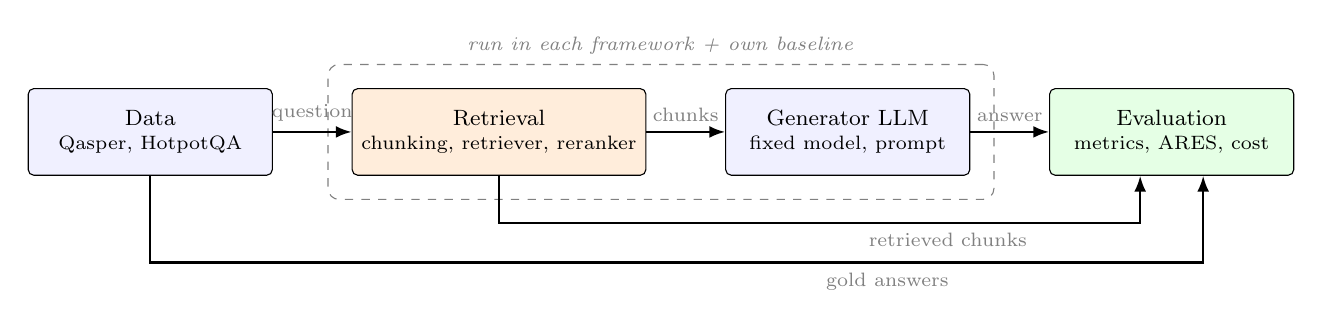
\begin{tikzpicture}[
  node distance=10mm,
  box/.style={draw, rounded corners=2pt, minimum height=11mm, minimum width=3.1cm, align=center, font=\footnotesize, fill=blue!6},
  var/.style={box, fill=orange!14},
  ev/.style={box, fill=green!10},
  arr/.style={-{Latex[length=2mm]}, thick},
  lab/.style={font=\scriptsize, gray, above}]
  \node[box] (data) {Data\\[-1pt]\scriptsize Qasper, HotpotQA};
  \node[var, right=of data] (ret) {Retrieval\\[-1pt]\scriptsize chunking, retriever, reranker};
  \node[box, right=of ret] (gen) {Generator LLM\\[-1pt]\scriptsize fixed model, prompt};
  \node[ev, right=of gen] (eval) {Evaluation\\[-1pt]\scriptsize metrics, ARES, cost};
  \draw[arr] (data)--(ret) node[lab,midway]{question};
  \draw[arr] (ret)--(gen) node[lab,midway]{chunks};
  \draw[arr] (gen)--(eval) node[lab,midway]{answer};
  \draw[arr] (ret.south) -- ++(0,-6mm) -| ([xshift=-4mm]eval.south) node[lab,below,pos=0.35]{retrieved chunks};
  \draw[arr] (data.south) -- ++(0,-11mm) -| ([xshift=4mm]eval.south) node[lab,below,pos=0.35]{gold answers};
  \begin{scope}[on background layer]
    \node[draw=gray, dashed, rounded corners, fit=(ret)(gen), inner sep=3mm,
          label={[font=\scriptsize, gray]above:\emph{run in each framework + own baseline}}] {};
  \end{scope}
\end{tikzpicture}
\caption{Experimental pipeline. The orange stage is varied in a grid; blue stages are fixed. Each framework is run on the identical grid with the same data and metrics. Retrieval metrics use the retrieved chunks, answer metrics, ARES and cost use the generated answers. Baselines (no retrieval, BM25 only) are described in the text.}
\label{fig:pipeline}
\end{figure*}

\subsection{Metrics}
\begin{itemize}
    \item \textbf{Retrieval:} Recall@5 (primary), MRR, nDCG@10.
    \item \textbf{Answer:} exact match and token F1 (primary).
    \item \textbf{Faithfulness:} ARES score \cite{ares}, the same evaluator for all frameworks (not Haystack's built-in ones), checked against about 150 items labelled by the team (Cohen's $\kappa$) and used only if $\kappa\ge0.6$.
    \item \textbf{Cost:} latency, peak memory and tokens per query.
    \item \textbf{Aggregation:} macro-average per dataset and split; failures score 0.
    \item \textbf{Uncertainty:} mean $\pm$ std over at least 3 seeds with 95\% bootstrap confidence intervals; a difference between frameworks is claimed only if the interval excludes 0.
\end{itemize}

\subsection{Success deliverables}
\begin{itemize}
    \item \textbf{D1:} one reproducible repository running at least 2 frameworks and 2 baselines on at least 2 datasets over the full grid with at least 3 seeds, from which a stranger reproduces one result using the README alone.
    \item \textbf{D2:} a quantified answer to H1--H3 (effect sizes with intervals), a decision rule (``use a framework / use plain RAG / skip retrieval'') and an error analysis of at least 20 failures grouped into named types.
\end{itemize}

\subsection{Work plan and owners}
Jan owns the pipeline core, the grid runner, compute and the Haystack adapter; Karolina the data, the RAGFlow adapter, literature and error analysis; Anna the metrics, ARES, statistics and the report. Each result is reviewed by the next person in the cycle Jan $\rightarrow$ Karolina $\rightarrow$ Anna $\rightarrow$ Jan. Table~\ref{tab:plan} gives the week-by-week plan.

\begin{table*}[t]
\centering\footnotesize
\setlength{\tabcolsep}{4pt}
\begin{tabular}{@{}>{\raggedright\arraybackslash}p{2.7cm}>{\raggedright\arraybackslash}p{4.1cm}>{\raggedright\arraybackslash}p{4.1cm}>{\raggedright\arraybackslash}p{4.1cm}@{}}
\toprule
\textbf{Week} & \textbf{Jan} & \textbf{Karolina} & \textbf{Anna}\\
\midrule
W1: 5--11 Nov & repository, config schema, Haystack pipeline end to end on 5 questions & Qasper and HotpotQA loaders, fixed seeded question lists & metric code (token F1, exact match, Recall@5, MRR, nDCG@10), unit tests on toy data\\
\addlinespace
W2: 12--18 Nov\newline\textit{18 Nov: mid-term video} & BM25-only baseline; proof of concept: Haystack and BM25 on 50 Qasper questions with token F1 and latency & Qasper evidence-to-chunk mapping, EDA start, literature table & video script and recording; check on a sample of 50 Qasper questions that the shared index retrieves the right paper\\
\addlinespace
W3: 19--25 Nov\newline\textit{25 Nov: Q\&A} & no-retrieval baseline; \textbf{budget estimate} (calls, hours, cost) for the full grid & RAGFlow adapter (pair session with Jan) & ARES setup and judge training; rebuttal; draft analysis plan (tests, variance method for H2)\\
\addlinespace
W4: 26 Nov--2 Dec\newline\textit{2 Dec: report} & pilot grid (10\% of questions, 1 seed) for both frameworks; runner resumes after failure; README draft & parity check of both frameworks and the own baseline under the matched configuration (H2); EDA report; revised literature & \textbf{freeze analysis plan} (tag in repo: metrics, tests, variance method); report\\
\addlinespace
W5: 3--9 Dec\newline\textit{9 Dec: feedback meeting} & launch the full grid, seed 1, Qasper & sample 150 items for ARES labelling (stratified over frameworks, disjoint from calibration); label & label the same items independently; ARES calibration on the disjoint set\\
\addlinespace
W6: 10--16 Dec & full grid, seed 1, HotpotQA; first sanity table & error analysis on seed-1 outputs, draft of failure types & $\kappa$ computed; \textbf{gate 16 Dec}: ARES used only if $\kappa\ge0.6$; dry run of the statistics on seed 1\\
\addlinespace
W7: 17--23 Dec & seeds 2--3 launched; cost measurements on an idle machine & at least 20 failures grouped into named types & statistics on seed 1; draft tables and figures for H1--H3\\
\addlinespace
W8: 24--30 Dec & buffer: runs continue unattended, Jan monitors & light drafting, no deadline: related-work text from the literature table & backup for the runs\\
\addlinespace
W9: 31 Dec--6 Jan\newline\textit{6 Jan: results freeze} & seeds finished, reruns of failures, tag the frozen results & error analysis finalised on the frozen results & final statistics: effect sizes, intervals, decision rule\\
\addlinespace
W10: 7--13 Jan\newline\textit{13 Jan: report, video, Q\&A} & final README; stranger test (a classmate reproduces one result); demonstration notebook & final literature, quiz, check of the data statement, error-analysis section & report, slides, video, LLM declaration, contribution table\\
\addlinespace
W11: 14--20 Jan\newline\textit{20 Jan: rebuttals} & own answers to final Q\&A & own answers to final Q\&A & own answers to final Q\&A\\
\bottomrule
\end{tabular}
\caption{Weekly plan with named owners, aligned with the course deadlines (in italics). D1 and D2 are due on 13 Jan. Everyone logs hours weekly for the contribution table.}
\label{tab:plan}
\end{table*}


\section{Contribution table}
\begin{tabular}{ |p{3cm}|p{3cm}|p{1cm}| } 
\hline
Student & Work & Hours \\
\hline
Jan Czemko & Solution concept and plan & 3h \\ 
Karolina Móżdżyńska & cell5 & cell6 \\ 
Anna Piórkowska & Introduction, Data, RAGFLow and DSPy & 4h \\ 
\hline
\end{tabular}

\section{Declaration of LLM use}
AI was used for creating LaTeX tables and figures, as well as general spell checking and grammar correction/improvment. It was used to search for literature and sources of knowledge.


% \\Detailed description (\textbf{max. 4 meaningful pages}) in English, including the following information:
% \begin{enumerate}
% \item scientific goal of the project (description of the problem to be solved, research questions and hypotheses);
% \item significance of the project (state of the art, justification for tackling a specific scientific problem, justification for the pioneering nature of the project, the impact of the project results on the development of the research field and scientific discipline);
% \item concept and work plan (general work plan - with a timeline, specific research goals, results of preliminary research, risk analysis);
% \item approach \& research methodology (underlying scientific methodology, methods, techniques and research tools, methods of results analysis, equipment and devices to be used in research);
% \item well-justified project literature (a reference list for publications included in the project description, with full bibliographic data);
% \item \textbf{data statement} (new for 2026/27) -- source of the data, licence, whether it contains personal data, and what you do about it. Six lines are enough;
% \item \textbf{contribution table} -- each team member, what they did, workload in hours. \textbf{Required in this and every later phase report; a report submitted without it is not accepted for grading, not just marked down};
% \item \textbf{declaration of LLM use} -- which tools, for what. \textbf{A report without this is not accepted for grading} (new for 2026/27).
% \end{enumerate}

% \textbf{Reminder: place this and every later submission in a folder named \texttt{surname\_surname\_surname\_surname} (all team members). The order set here must not change for the rest of the semester -- a mismatch costs 5 points.}


\begin{thebibliography}{10}
\bibitem[Dasigi et al., 2021]{dasigi2021qasper}
Pradeep Dasigi, Kyle Lo, Iz Beltagy, Arman Cohan, Noah A. Smith, and Matt Gardner. 2021.
A Dataset for Question Answering on Scientific Papers. In \emph{NAACL-HLT 2021}.

\bibitem[Yang et al., 2018]{yang2018hotpotqa}
Zhilin Yang, Peng Qi, Saizheng Zhang, Yoshua Bengio, William W. Cohen, Ruslan Salakhutdinov, and Christopher D. Manning. 2018.
HotpotQA: A Dataset for Diverse, Explainable Multi-hop Question Answering. In \emph{EMNLP 2018}.

\bibitem[Brown et al., 2025]{brown2025}
Andrew Brown, Muhammad Roman, Barry Devereux. 2025.
A Systematic Literature Review of Retrieval-Augmented Generation: Techniques, Metrics, and Challenges. 

\bibitem[Saad-Falcon et al., 2024]{ares}
Jon Saad-Falcon, Omar Khattab, Christopher Potts, Matei Zaharia. 2025.
ARES: An Automated Evaluation Framework for Retrieval-Augmented Generation Systems.

\bibitem[Pietsch et al., 2024]{haystackdocs}
Pietsch, M., Soni, T., Chan, B., Möller, T., Kostić, B. 2020. 
Haystack. GitHub. https://github.com/deepset-ai/haystack

\bibitem[InfiniFlow, 2024]{ragflow}
InfiniFlow. 2024. GitHub. https://github.com/infiniflow/ragflow 

\bibitem[Stanford NLP, 2024]{dspy_repo}
Omar Khattab, Stanford NLP.
DSPy: The Framework for Programming—Not Prompting—Language Models.
GitHub. https://github.com/stanfordnlp/dspy.

\bibitem[Stanford NLP, 2024]{dspy_docs}
Omar Khattab, Stanford NLP.
DSPy Documentation: Program, Don't Prompt, Your LLMs.
https://dspy.ai/current/.

\end{thebibliography}


% include your bib file like this:
%\bibliographystyle{acl}
%\bibliography{acl2015}

\end{document}